\section{Getting to Know Your Equipment}
\label{lab_equipment}

%\makelabheader %(Space for student name, etc., defined in master.tex)

\bigskip

\textbf{Resistors}
\begin{enumerate}[wide]

\item Using the resistor color code described in Appendix \ref{resistor_code}, what colors should the bands be to indicate $1\kohm$ on a four-band resistor?  What about on a five-band resistor?  Make predictions first, then check  the actual colors on the two different kinds of $1\kohm$ resistors in the plastic boxes at your lab station.

\item What are the apparent tolerances of your four-band and five-band $1\kohm$ resistors, and how do you know?

\item All of the five-band resistors in your kits have the same color tolerance band (brown).  They also happen to have the same color on their third bands.  What color is it, and what does that mean?
 
\bigskip
\textbf{Digital Multimeters}

\item \label{part_150_ohm_measurements} Use your digital multimeter (DMM) to measure the resistances of a 150 $\Omega$ and a 150 k$\Omega$ resistor from your kit.  How close are they to their stated values?   

\item What does the ``range'' button do on your DMM?  What is ``auto ranging'' and how do you get it to do that?  What might be an advantage to setting a fixed manual range vs. auto ranging?

\item What is the claimed accuracy of your DMM for the resistance readings in part \ref{part_150_ohm_measurements}?  To find this out, you will need to look in the paper manual for your DMM.  It will specify that the maximum error is the sum of a percentage of the reading \textit{plus} some number of ``digits,'' meaning the least significant digit on the display.  (That is, if your diplay reads $12.35\kohm$, then ``$\pm 4$~DGTS would mean $\pm 4 \times 0.01\kohm$, or $\pm 40\ohm$.)   The fixed number of digits is called the \textit{offset error}.

\item The offset error listed in the manual is probably a wild overstatement of the actual offset in your DMM. To test this, you can short circuit the two resistance inputs together to approximate a resistance of $0\ohm$ and measure the resistance on all possible ranges. What is the \textit{actual} offset error of your DMM for resistance measurements?  You can do the same thing to measure the offset in DC voltage measurements.  What do you find there? 

\item Measure the resistance of yourself.  Does it make a difference if you lick your fingers?  

\item What does the min/max/avg button on the DMM do?

\item The yellow button on your DMM acts as a \button{SHIFT} key to select any function marked in yellow on the main selector dial.  For instance, when measuring resistance, the yellow button activates ``continuity'' mode, denoted by the  ``\raisebox{-0.8 ex}{
\includegraphics[height=0.2in]{equipment/sound.pdf}}'' symbol.  What does continuity mode mean, and when might it be useful? \label{part_audible_dmm}  Also, what does the ``$\sim$'' symbol mean when measuring voltage or current?

\end{enumerate}


\bigskip

\begin{minipage}{.70\textwidth}
\textbf{PB-505A Circuit Trainer and Breadboard}
\medskip


Most of the circuit building you do this semester will be on the big blue \mbox{PB-505} at your lab station, which combines several useful functions like DC voltage sources, a function generator, and various switches and indicators with a large empty area called a \textit{breadboard} for prototyping circuits. The breadboard area has repeating rows and columns of holes for connecting small components like resistors, integrated circuits (ICs), and jumper wires.  
\end{minipage}
\begin{minipage}{.29\textwidth}
\hfill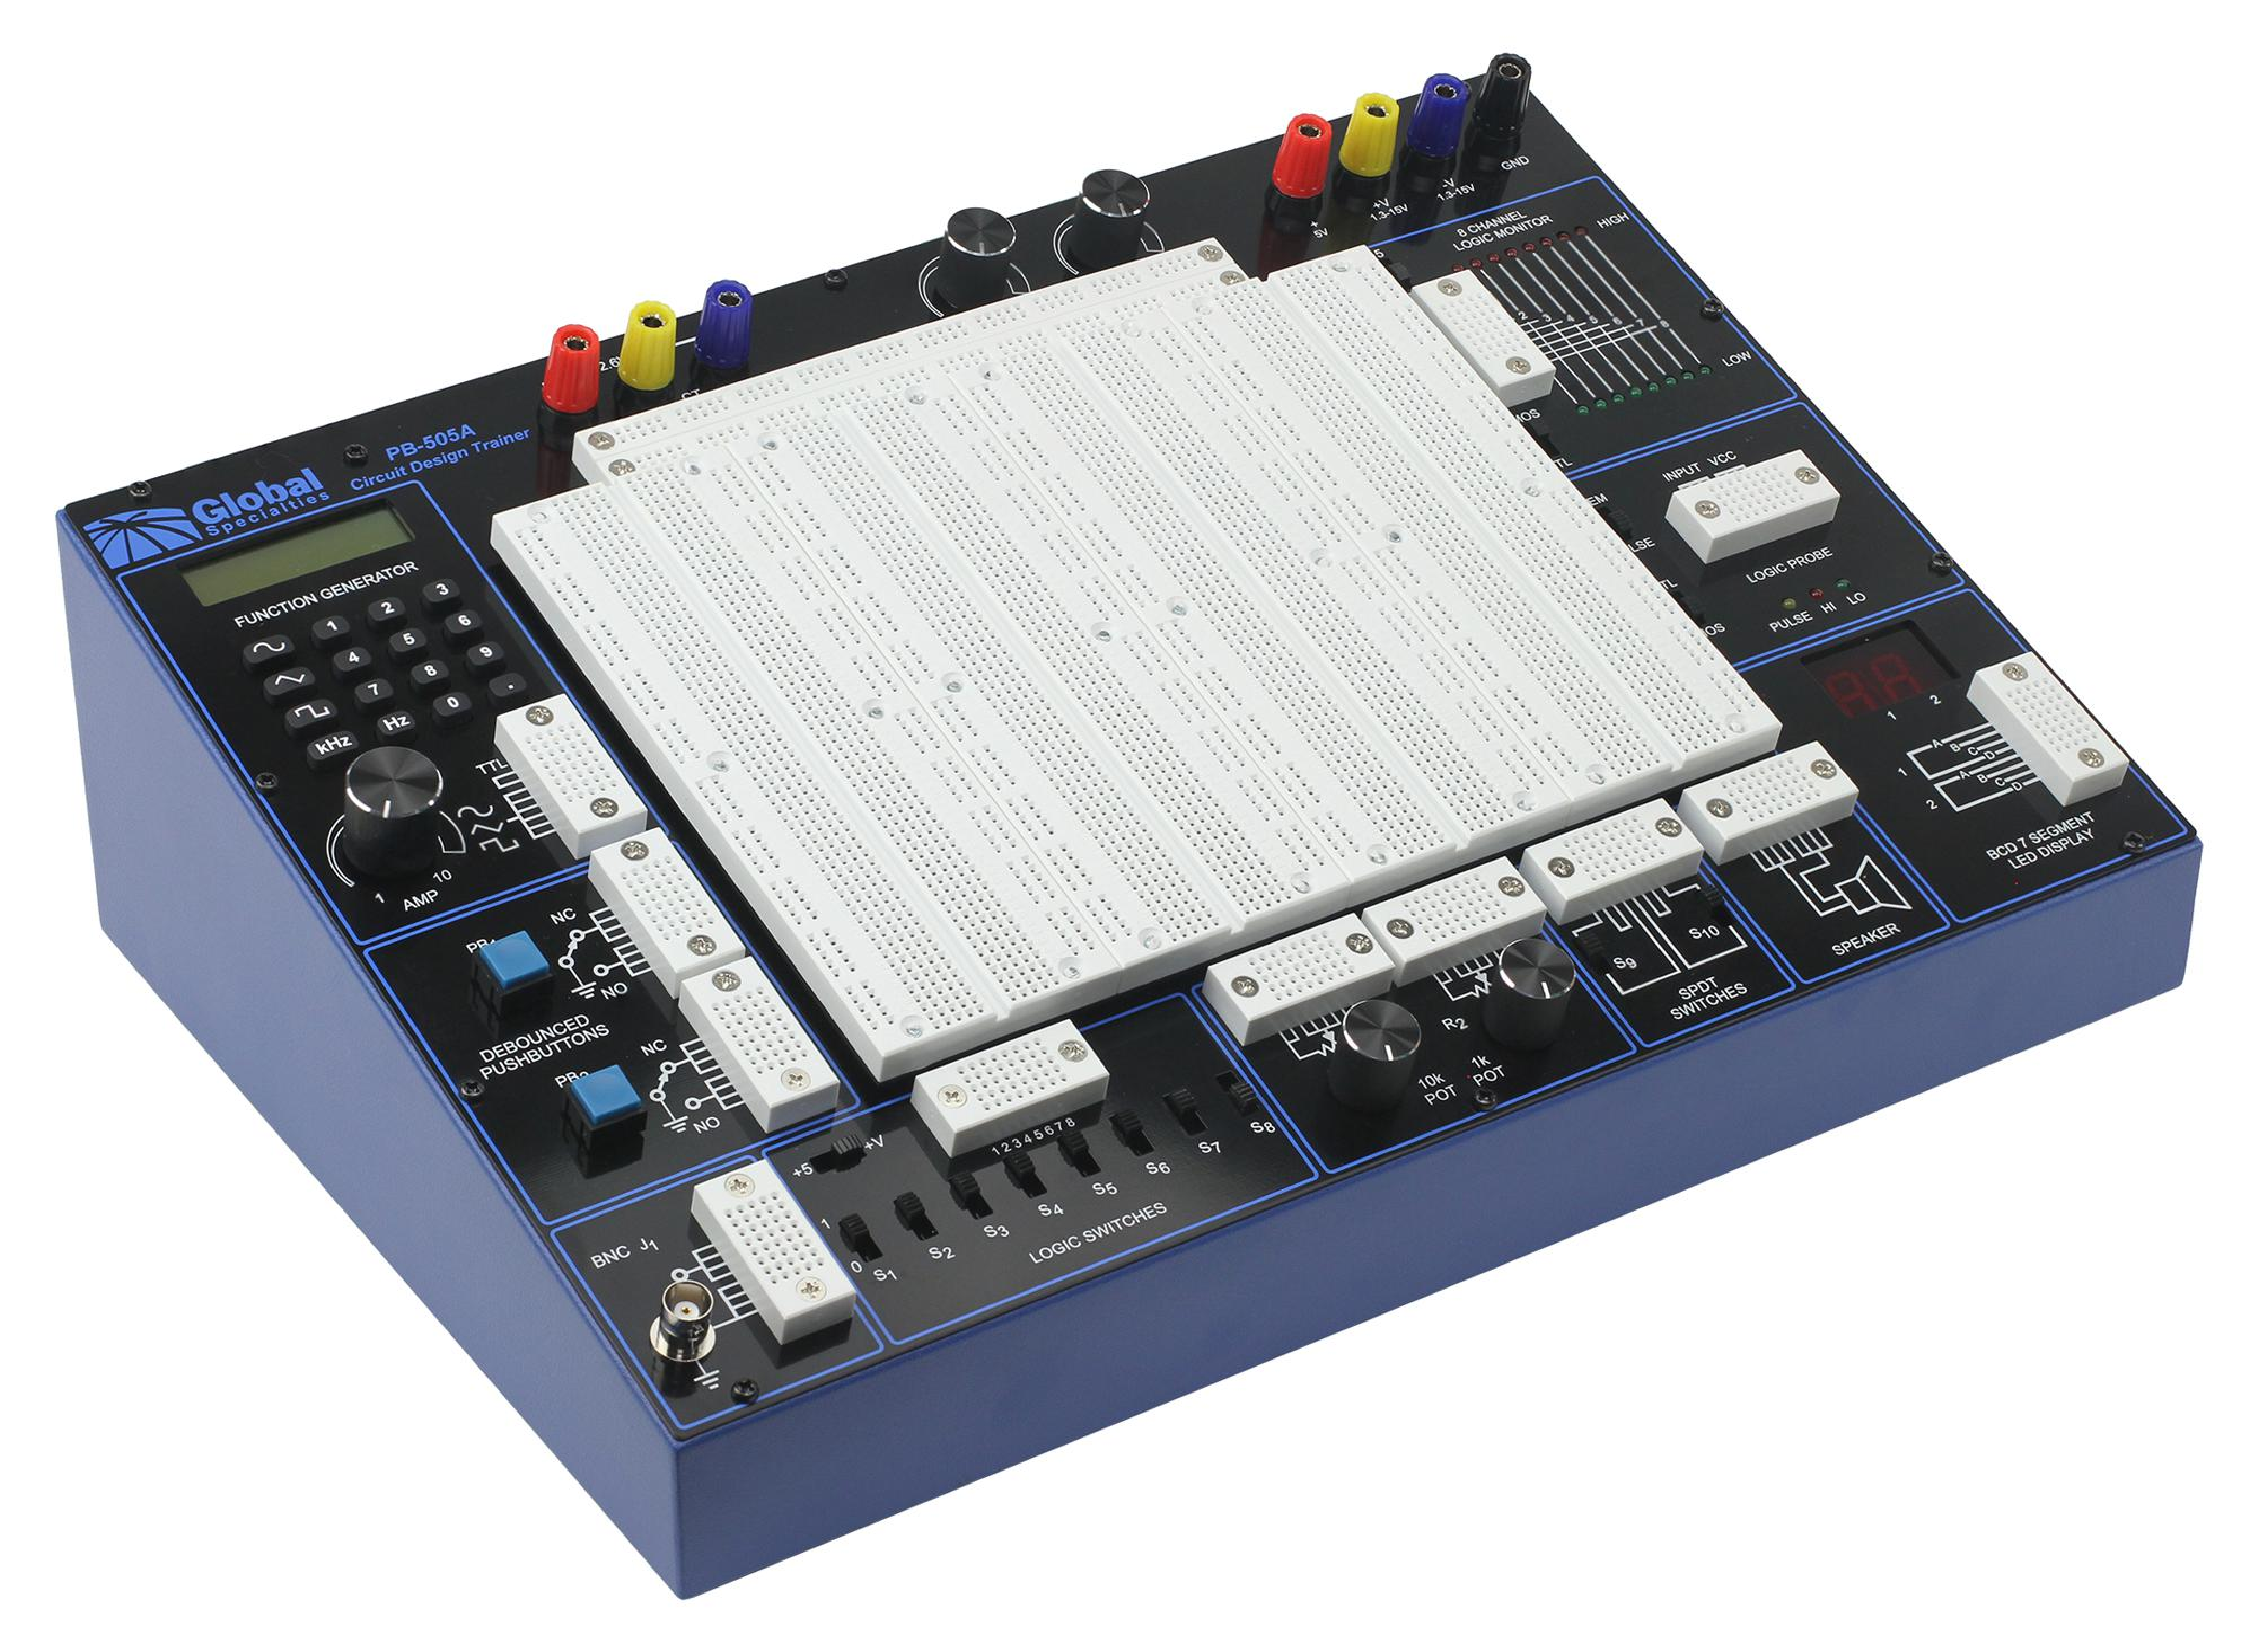
\includegraphics[width=0.92\linewidth]{equipment/PB-505A.pdf}
%\caption*{PB-505A trainer}
\end{minipage}

\pagebreak[3]
In this part, you'll use the continuity mode you discovered in part \ref{part_audible_dmm} to figure out which holes on your ``breadboard'' are connected to each other.  The regular probes for your DMM are too big to fit in the breadboard holes, so the best way to connect the two is to use a banana cable, alligator clip, and a long jumper wire.

\begin{center}
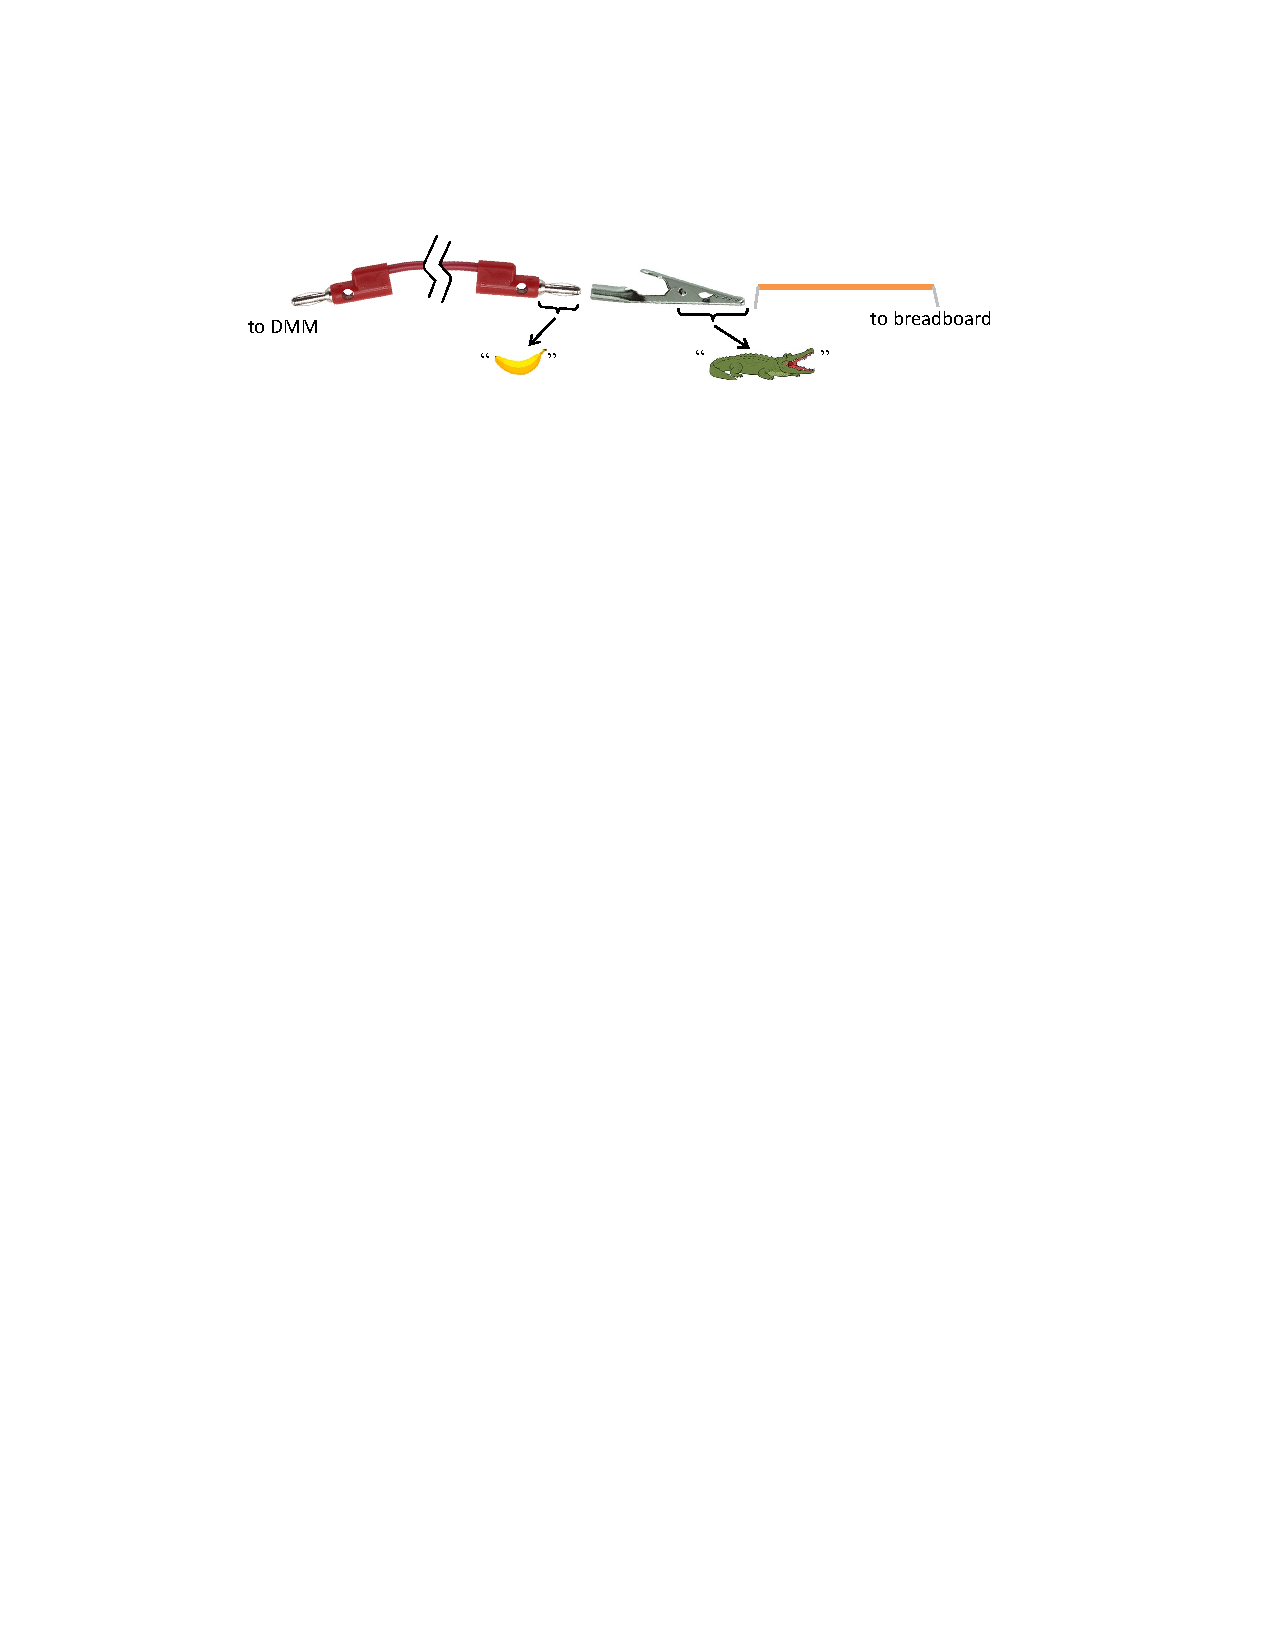
\includegraphics{equipment/breadboard_connection.pdf}
\end{center}


\begin{enumerate}[wide,resume]

\item The picture on the right is similar to the breadboard on your \mbox{PB-505} trainer but its rows and columns are labeled.  Use your DMM to measure the corresponding parts of your breadboard: 

{ %start of block defining \redplus and \blueminus
\newcommand{\redplus}{\textbf{\textcolor{red}{+}}}
\newcommand{\blueminus}{\textbf{\textcolor{cyan}{--}}}

\begin{minipage}{.65\textwidth}
\begin{itemize}[nosep]
\item In the middle sections, are the holes 1a through 1e connected to each other?  What about holes 1a through 1j? 
\item Is hole 1a connected to anything in row 2? Or to any other rows?
\item Along the sides, there are vertical groups of five holes in columns labeled ``\redplus'' and ``\blueminus''.  Are all groups of five in the ``\redplus'' column connected to each other vertically?  (Be sure to check the entire length of the column!)  
\item Are any holes in the ``\redplus'' column connected to the ``\blueminus'' column?  Are the two ``\redplus'' columns on either side connected to each other?
\end{itemize}
\smallskip
In addition to answering the specific questions above, make a quick, labeled sketch in your lab notebook showing which holes are connected to each other.
\end{minipage}
\begin{minipage}{.34\textwidth}
\hfill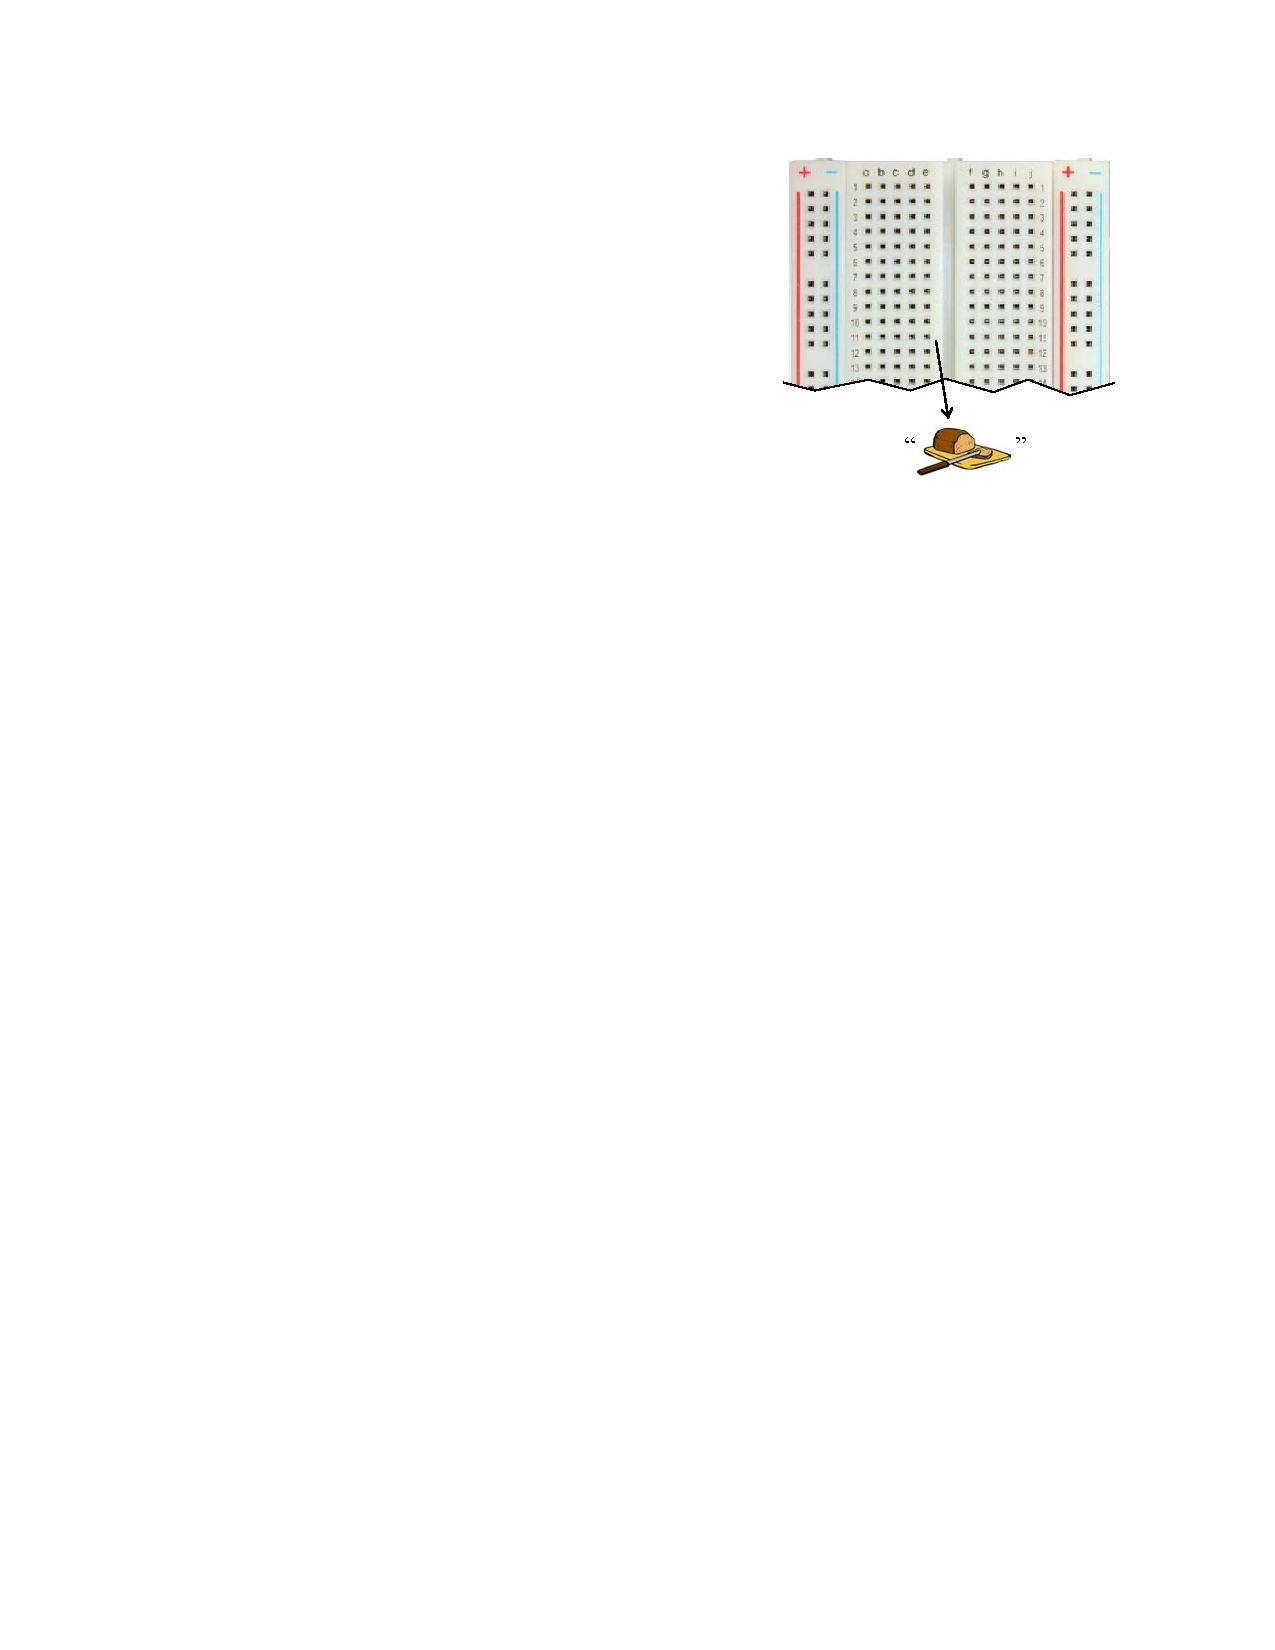
\includegraphics[width=0.9\linewidth]{equipment/breadboard_section.pdf}
%\caption*{PB-505A trainer}
\end{minipage}

} %end of block defining \redplus and \blueminus

\bigskip
\textbf{About ``Ground''}

There are at least three different circuit symbols that are commonly referred to as ``ground'' but which actually mean slightly different things:

\begin{description}[labelindent=0.25in, leftmargin=0.5in]

\item[Common 
(\raisebox{-0.8 ex}{
\includegraphics{equipment/common_symbol.pdf}}):] 
For convenience we usually define one place in a circuit to be at zero potential---often the negative terminal of a battery or power supply.  In complicated circuits, using the triangle symbol for ``common'' makes circuit diagrams tidier than drawing a spaghetti tangle of lines back to the power supply.  In specific cases it can be called ``signal common'' or ``digital common,'' but it's also often just called ``ground''.

\item[Chassis Ground
(\raisebox{-0.8 ex}{
\includegraphics{equipment/chassis_symbol.pdf}}):] 
A \textit{chassis} (which, perplexingly, is pronounced to rhyme with ``gassy'') is an object's metal frame or metal enclosure.  Using the chassis itself as a part of the electrical circuit can reduce the amount of wiring needed---hey, if it conducts and it's already there, we might as well use it! Connecting the chassis to Earth ground also helps block electromagnetic interference and can protect anyone touching the chassis from electric shock.

\item[Earth Ground
(\raisebox{-1.0 ex}{
\includegraphics{equipment/earth_symbol.pdf}}):] 
The common and/or the chassis ground are often physically connected to the Earth---which for many buildings literally means a metal spike driven into the ground.  Within the building, the connection from the Earth to the chassis ground is made through the electrical outlets using the third prong of the power cord.

\end{description}


Although the three circuit symbols above are supposed to mean different things, in practice the distinctions between them are often ignored---as they are for many other circuit symbols as well.  You should make at least some effort to use the right one yourself, but be aware that others (including your instructor!) may use them interchangeably.

\item If you look on the back of your \mbox{PB-505}, you'll see a small screw  just above the power cord with a green wire connected to it.  That screw terminal is the electrical connection to the chassis, and it's even labeled with the chassis ground symbol.  Is the chassis ground also an Earth ground when the unit is plugged in?

\pagebreak[3]
\item The black banana jack at the top right corner of your \mbox{PB-505}  is labeled ``GND''.  On the opposite corner, the connector labeled ``BNC J1'' is also marked to show that its outer, silver shell is connected to Earth ground.  Are these two points connected to each other?  And are either of them actually connected to the Earth when the unit is plugged in?  What would be the easiest way to connect and disconnect the ``GND'' banana jack to Earth ground as needed?

\item The red banana jack near ``GND'' is a +5-volt DC voltage source, or \textit{power supply.}  What is that ``+5 volts'' relative to?  Measure the actual voltage of your 5-volt supply, including an uncertainty range based on the stated accuracy of your DMM.  Are you able to rule in or rule out the possibility that the +5 V supply is exactly 5.0000 volts?  

\item While you're at it, use your DMM to measure the actual ranges of the variable voltage supplies on your \mbox{PB-505}, which are the yellow and blue banana jacks labeled +V and $-$V.  Are their ranges exactly 1.3 to 15.0 volts when you turn the knobs?

\vfill
\bigskip\bigskip
\textbf{Possible Exam Questions:}

(\textit{These questions are optional things for you to think about; you don't need to put them in your lab notebook, and I won't be checking them.})

\begin{itemize}
\item You have a 5~V source, and you would like to build a simple voltage divider using two equal resistors to give an output of 2.5 volts.  The 2.5 volt signal will go to an amplifier with an input impedance of about 50~k$\Omega$.  What value resistors should you use for your voltage divider: 1~k$\Omega$, 50~k$\Omega$, or 1~M$\Omega$?

\item Describe how to use the resistor color code

\item From memory, what is the approximate input impedance of your DMM when it is used as a voltmeter?  What is the approximate input impedance of your DMM when it is used as an ammeter on the 10~mA scale?  On the 10~A scale?  (Knowing real-life approximate values of things is important, and asking you them on an exam is totally fair game.)

\item From memory, what is the approximate accuracy of your DMM?  (Knowing real-life approximate values of things is important, and asking you them on an exam is totally fair game.)

\item What are the precise meanings of \textit{common, chassis ground,} and \textit{Earth ground?}
\end{itemize}


%--------------------------------------------------------------------
\begin{comment}

\begin{minipage}{.75\textwidth}

\item A ``single pole double throw'' (SPDT) switch has three terminals, as shown in the diagram to the right.  The switches S9 and S10 on your proto boards each have eight little holes for wire connections; the leftmost two are always connected to each other, as are the rightmost two and the four in the center.  Which of these sets of holes correspond to each of the three terminals?  Which holes are connected to each other when the switch is up, and when it is down?  Make a good diagram in your lab notebook; you'll need to know how to use these later! \label{part_switches}
\end{minipage}
\begin{minipage}{.24\textwidth}
%\center{
\includegraphics[width=0.9\textwidth]{equipment/spdt.eps}}
\center{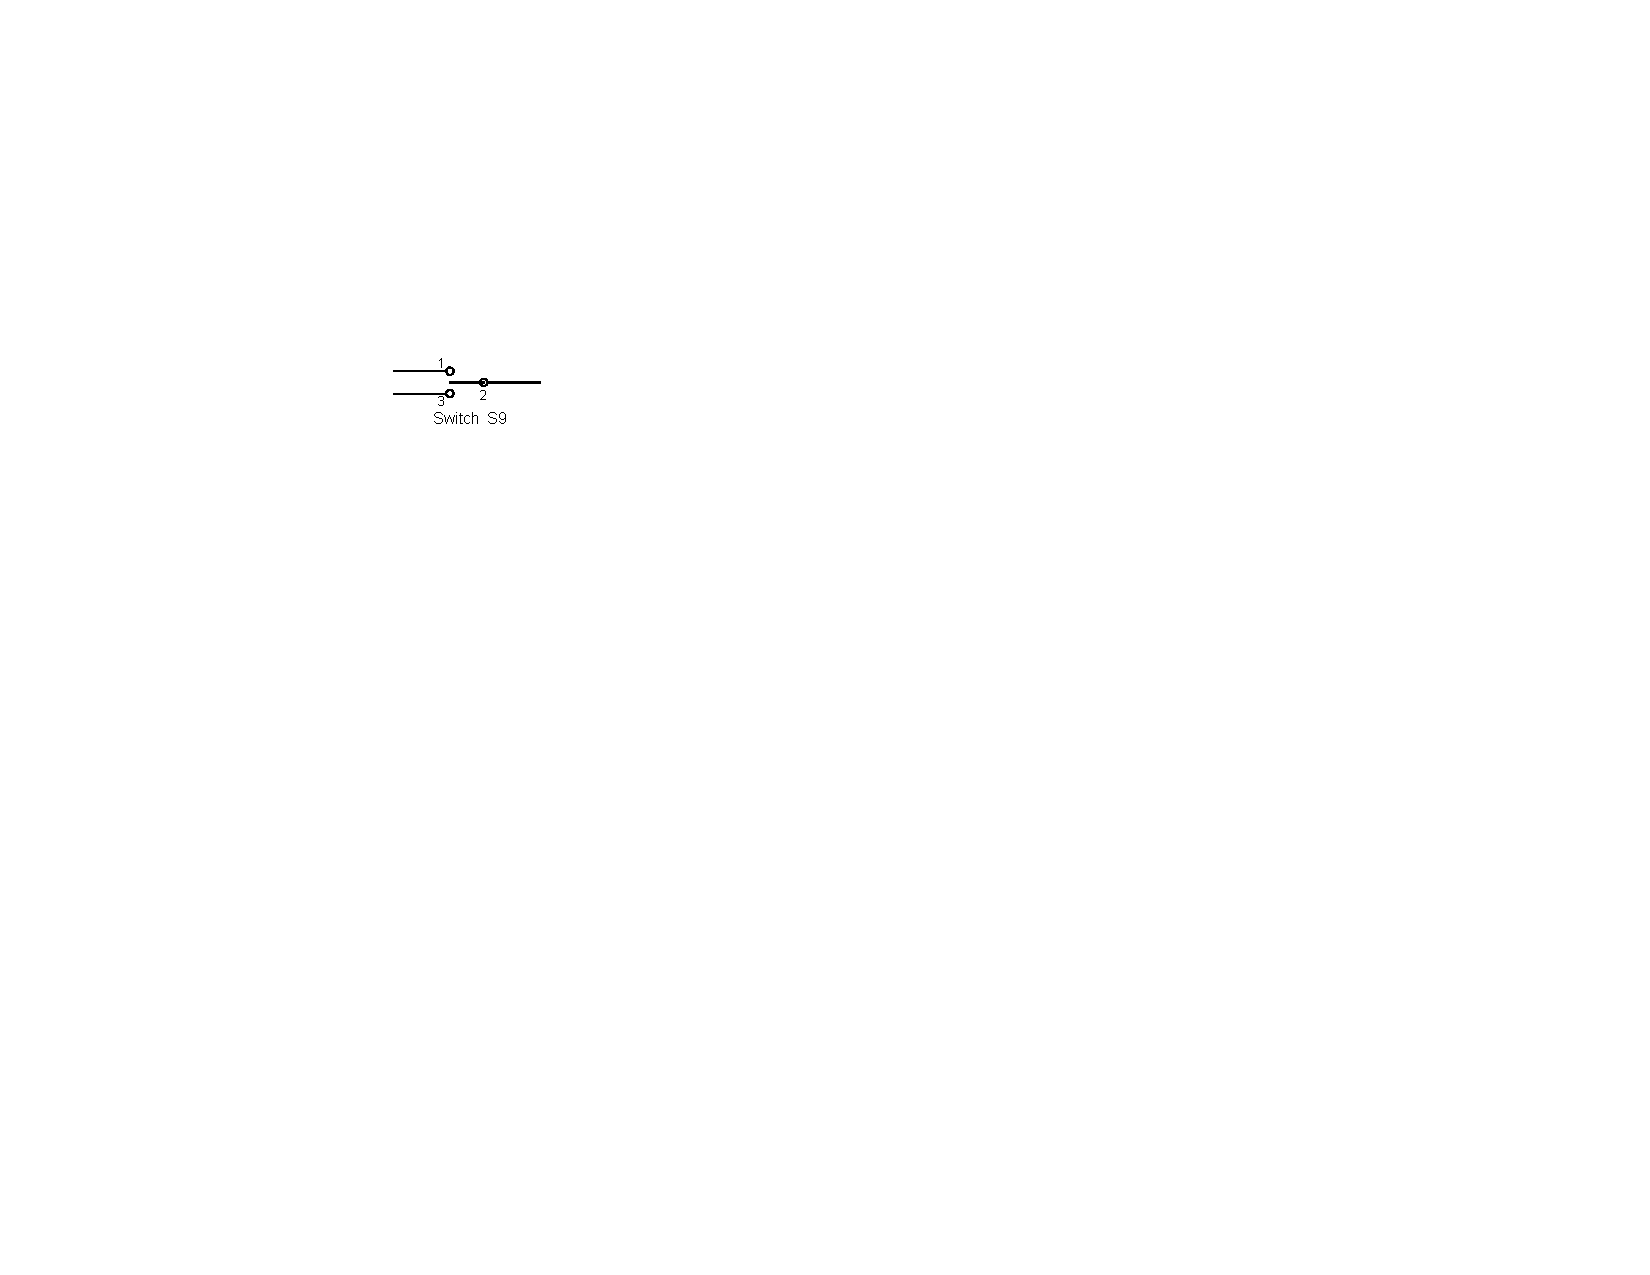
\includegraphics{equipment/spdt2.pdf}}
\center{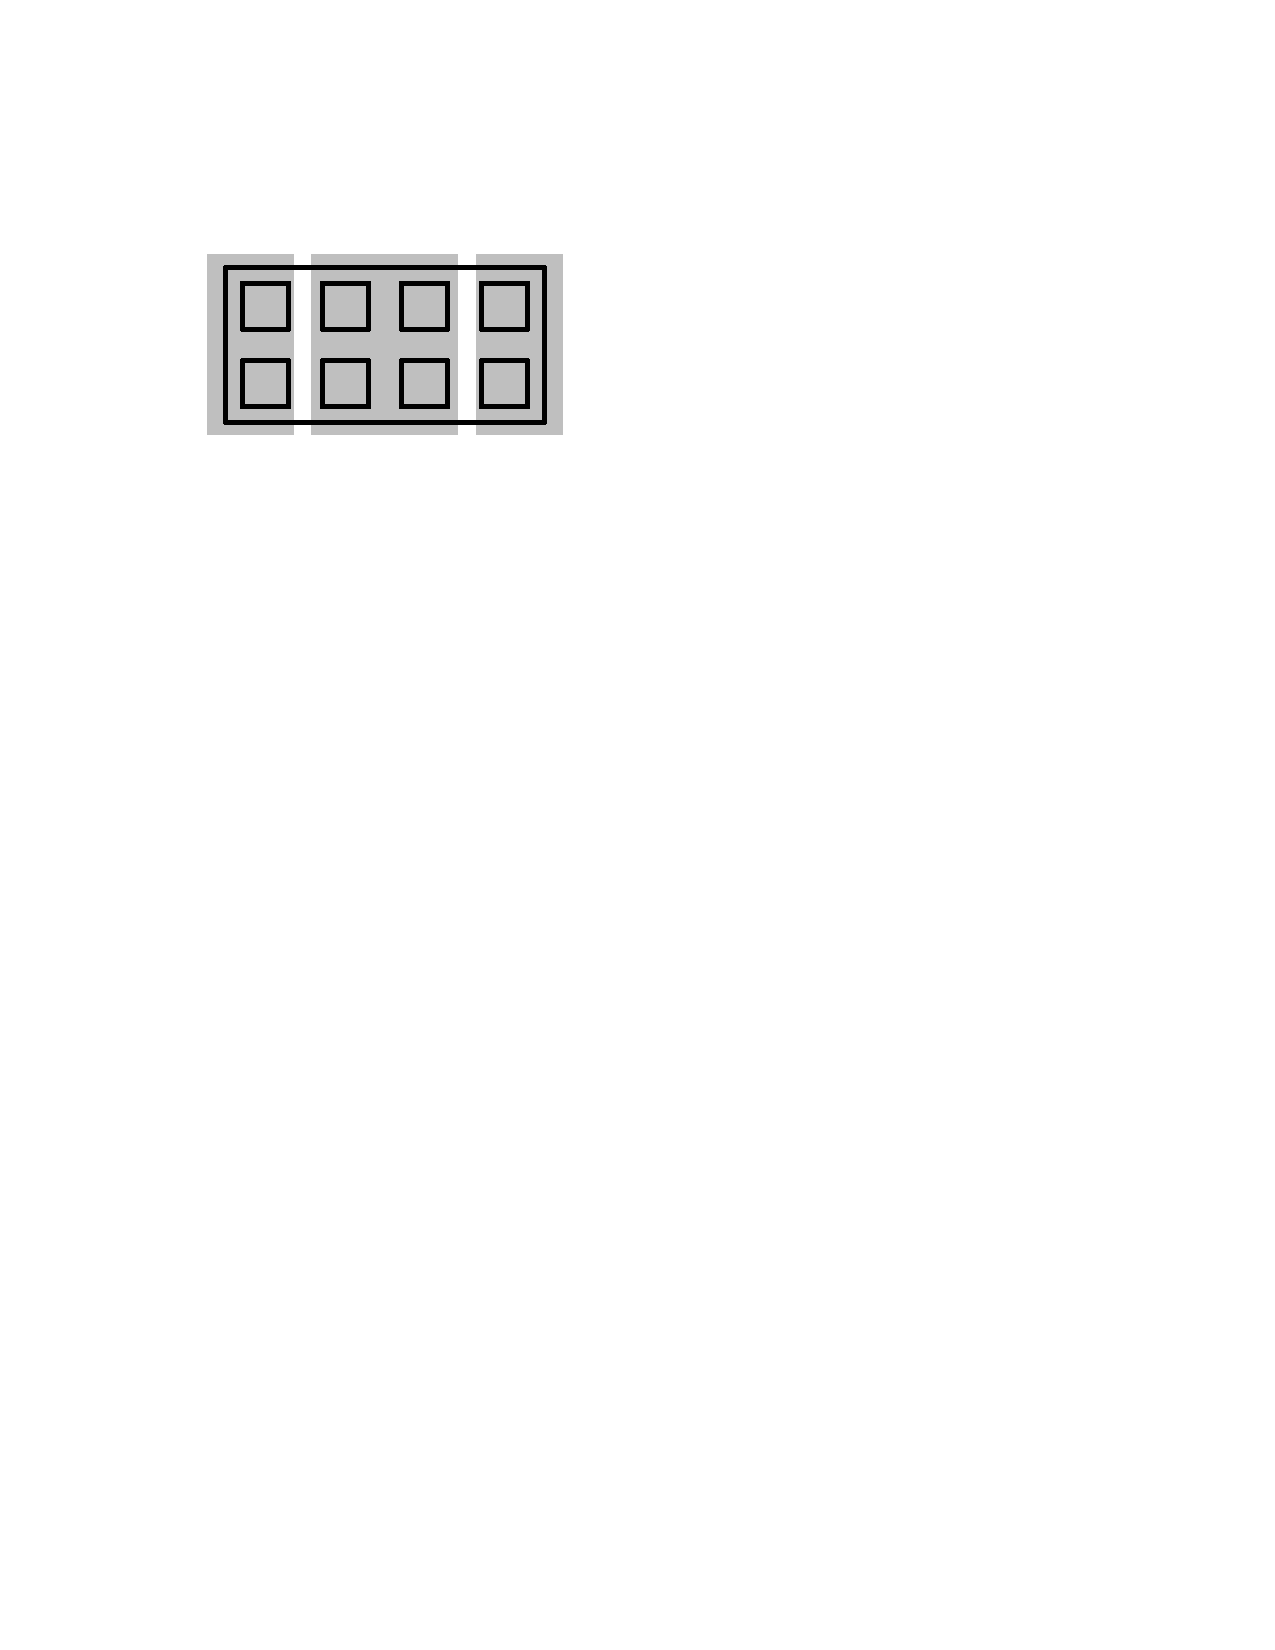
\includegraphics[width=0.7\textwidth]{equipment/spdt_contacts.pdf}}
\end{minipage}

\item Use your DMM to measure the resistance of the switch when it is closed.  If you can't make an accurate measurement, can you at least set an upper limit on the resistance? 



\item Set your function generator to a 1.0 kHz sine wave, and use your DMM to measure the frequency and amplitude of the oscillating voltage with the amplitude slider all the way up.   As with your 5~V supply, you will be measuring the voltage between the function generator's output and ground.  Will that voltage be AC or DC?  (Note that the function generator has a block of eight holes for the output, similar to the switches S9 and S10.  In this case, the rightmost six are all connected together; that's the output you want.  The leftmost two are the ``TTL'' signal; you'll learn about that in Lab \ref{lab_oscilloscope}.)

\item Just for fun, let's hook up the function generator to your speaker.  The speaker has two terminals, one connected to the top four holes in the block of eight, and one connected to the bottom four holes.  One speaker terminal should connect to the function generator's output.  Where should the other terminal connect to?  Once you have it hooked up, what's the highest frequency you can hear?  How does that compare with the highest audible frequency for your teacher, who spent way too much time playing in really loud, bad rock bands in college?
 
\end{comment}
\end{enumerate}



